\documentclass[fleqn]{article}
\oddsidemargin 0.0in
\textwidth 6.0in
\thispagestyle{empty}
\usepackage{import}
\usepackage{amsmath}
\usepackage{graphicx}
\usepackage{flexisym}
\usepackage{calligra}
\usepackage{amssymb}
\usepackage{bigints} 
\usepackage[english]{babel}
\usepackage[utf8x]{inputenc}
\usepackage{float}
\usepackage[colorinlistoftodos]{todonotes}


\DeclareMathAlphabet{\mathcalligra}{T1}{calligra}{m}{n}
\DeclareFontShape{T1}{calligra}{m}{n}{<->s*[2.2]callig15}{}
\newcommand{\scriptr}{\mathcalligra{r}\,}
\newcommand{\boldscriptr}{\pmb{\mathcalligra{r}}\,}

\definecolor{hwColor}{HTML}{1a0252}

\begin{document}

  \begin{titlepage}

    \newcommand{\HRule}{\rule{\linewidth}{0.5mm}}

    \center


    \textsc{\LARGE Arizona State University}\\[1.5cm]

    \textsc{\LARGE Quantum Physics II}\\[1.5cm]


    \begin{figure}
      
\includegraphics[width=\linewidth]{asu.png}
    \end{figure}


    \HRule \\[0.4cm]
    { \huge \bfseries Problem Set 1}\\[0.4cm] 
    \HRule \\[1.5cm]

    \textbf{Behnam Amiri}

    \bigbreak

    \textbf{Prof: Onur Erten}

    \bigbreak


    \textbf{{\large \today}\\[2cm]}

    \vfill

  \end{titlepage}

  \begin{enumerate}
    \item \textbf{(2-8)} The ether-wind theory of the Michelson-Morely experiment is discussed in the text for 
    the special case where the arms of the inter-ferometer are parallel and perpendicular to the wind. Consider
    the general case for an angular setting $\theta$ as shown (see the figure). Prove that, for equal arms of length
    $l$, the time difference for the two paths is given to a good approximation by
    $$\delta t(\theta)=\dfrac{v^2 l}{c^3} cos(2 \theta)$$
    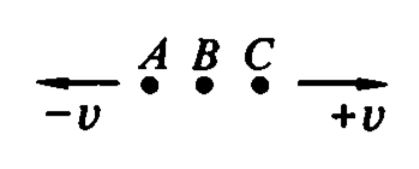
\includegraphics[height=4cm, width=4cm]{1.JPG}

      % \textcolor{hwColor}{

      % }

    \item \textbf{(3-4)} Given that 
    $$x^'=\gamma (x-vt)$$
    and 
    $$t^'=\gamma (t-\dfrac{vx}{c^2})$$
    derive the equations for $x$ and $t$ in terms of $x^'$ and $t^'$.

      % \textcolor{hwColor}{

      % }

    \item \textbf{(4-4)} Our galaxy is about $10^5$ light-years across, and the most energetic particles known
    have an energy of about $10^{19} ~ eV$. How long would it take a proton with this energy to traverse the galaxy
    as measured in the rest frame of 
    \begin{enumerate}
      \item The galaxy?

        % \textcolor{hwColor}{

        % }

      \item The particle?

        % \textcolor{hwColor}{

        % }

    \end{enumerate}

  \end{enumerate}

\end{document}